\section{Related Work}
\label{sec:related_work}

In preparation of creating an own Captcha service we searched the Internet for existing ideas and implementations of systems used for data labeling and machine learning purposes. The first popular approach was the Soylent Grid paper which was published in 2007 \footnote{http://vision.ucsd.edu/sites/default/files/icv2007.pdf}. Although there were never any popular implementations of the ideas, the paper provided several different approaches for data labeling. They were mostly based around the idea of object recognition in images, e.g. by clicking on objects or drawing rectangles around it. Other proposals were directed to object recognition, where users had to name objects displayed in certain images.\\
Another paper which was published just a year later, dealt with text recognition and described the concept which was implemented in reCAPTCHA v1 \footnote{http://science.sciencemag.org/content/321/5895/1465.full}. The system was created by Google in order to solve problems in the "Google Book Project). Two different optical character recognition (OCR) algorithms were used to translate images of scanned pages into digital texts. The solving of Captchas was used to identify words which could not be deciphered clearly by the OCR algorithms. Because of its detailed documentation and its successful usage this method was ideal to be implemented and therefore the first Captcha type which is supported by our system. \\
\begin{figure}[!h]
	\centering
	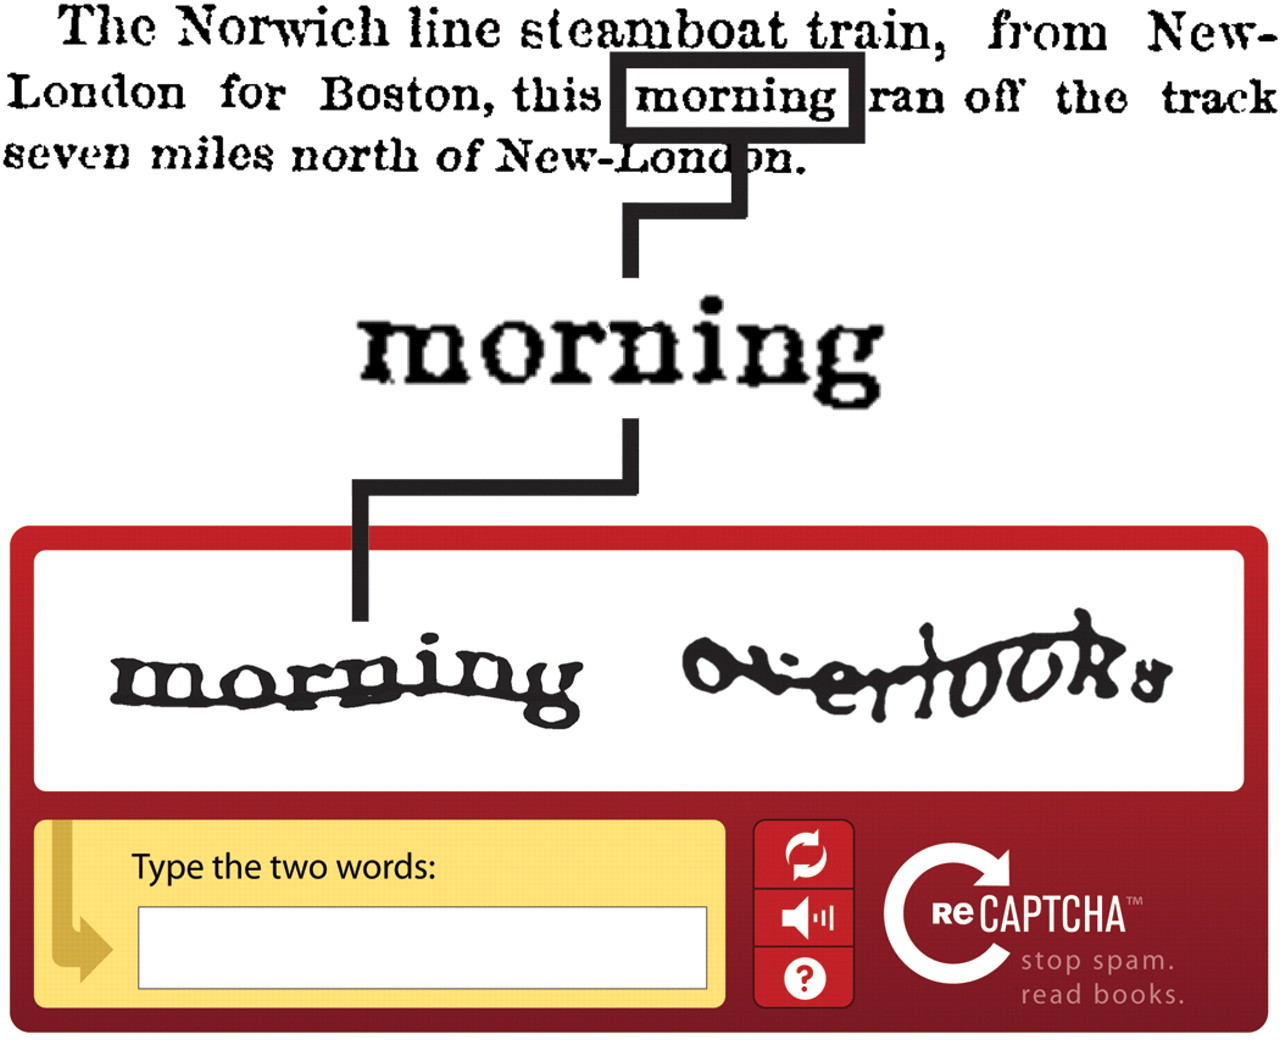
\includegraphics[width=0.4\linewidth]{content/figures/recaptcha.jpg}
	\caption{The reCAPTCHA approach explained in one picture}
	\label{fig:recaptcha}
\end{figure}
\clearpage